\begin{figure}[h]
\centering

\begin{subfigure}[b]{0.4\textwidth}
  \centering    
  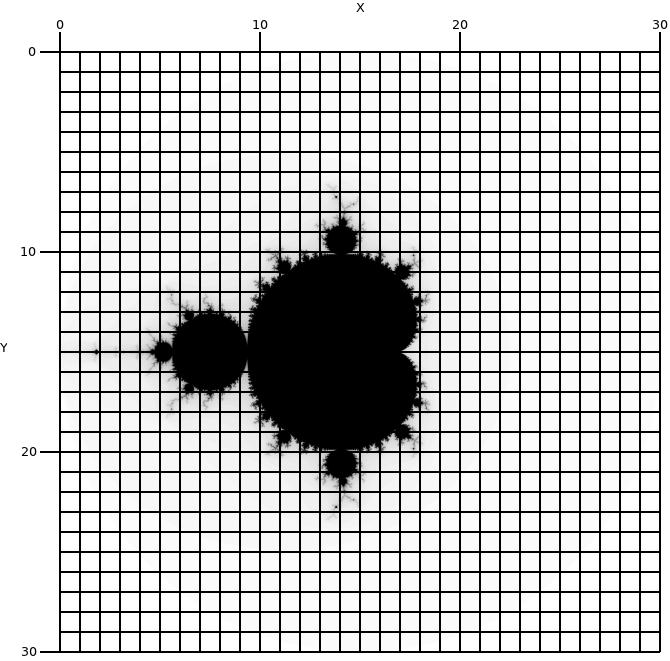
\includegraphics[width=\textwidth]{rasterplane}
  \caption{
     \tiny A representation of the points sampled on the complex plane.
  }
  \label{fig:rast-1}
\end{subfigure}
~ %spacer
\begin{subfigure}[b]{0.4\textwidth}
  \centering
  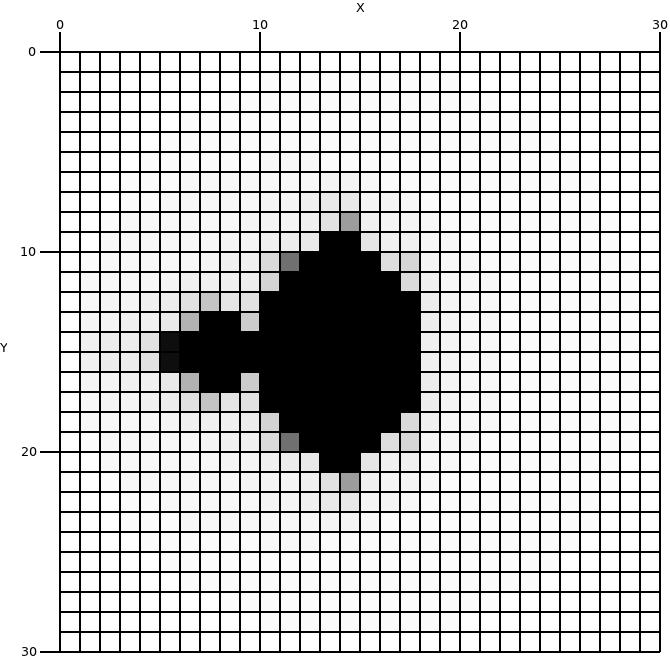
\includegraphics[width=\textwidth]{rastout}
  \caption{
     \tiny The result for the given raster plane after processing.
  }
  \label{fig:rast-2}
\end{subfigure}

% full caption
\caption{
    A visual representation of an example raster plane where HEIGHT and WIDTH equal
    thirty and MAX\_ITERATIONS equals seventy. Figure \ref{fig:rast-2} shows how the
    raster plane produces an approximation of the complex plane.
}
\label{fig:rasterdemo}
\end{figure}

